\section{正式实验结果}

\subsection{运行环境与数据规模}

正式实验在 Python 3.11.9、PyTorch 2.0.1、CUDA 11.8 和 cuDNN 8.7.0 环境中完成。
硬件为 NVIDIA GeForce GTX 1050 Ti，总显存 4096 MiB，含 6 个 CUDA 多处理器。
实验共使用 13320 个通过完整性校验的 UCF101 视频，其中 8476 个用于训练拟合，
1061 个用于验证，3783 个用于最终测试。

\subsection{三条主路线}

表~\ref{tab:main_results} 汇总三种子均值和样本标准差。每个均值都来自三次独立头部训练，
而不是对同一个模型的重复推理。

\begin{table}[H]
  \centering
  \caption{主路线正式结果}
  \label{tab:main_results}
  \resizebox{\textwidth}{!}{
  \begin{tabular}{lccccc}
    \toprule
    路线 & Top-1 & Top-5 & 峰值显存/MiB & 吞吐/(video/s) & 参数量/百万 \\
    \midrule
    R3D-18 基线 & 76.37±0.30\% & 94.48±0.08\% & 62 & 32.34 & 33.37 \\
    TSN-2D 线性 & 81.29±0.64\% & 95.89±0.19\% & 146 & 52.98 & 23.71 \\
    TSN-2D 时序注意力 & 82.70±0.54\% & 95.32±0.60\% & 990 & 52.98 & 23.71 \\
    R(2+1)D-18 & 83.97±0.26\% & 96.22±0.19\% & 62 & 22.20 & 31.51 \\
    \bottomrule
  \end{tabular}}
\end{table}

\begin{figure}[H]
  \centering
  \includegraphics[width=0.88\textwidth]{../../figures/main_route_accuracy.pdf}
  \caption{三条主路线的 Top-1 与 Top-5 准确率}
  \label{fig:main_results}
\end{figure}

TSN 的线性头已经达到 81.29\%，时位置注意力头提高到 82.70\%。R(2+1)D-18 取得
最高 Top-1 83.97\%，但特征提取吞吐为 22.20 video/s，明显低于 TSN 的 52.98
video/s。R3D-18 虽然吞吐居中，但 Top-1 只有 76.37\%，说明直接堆叠三维卷积并不能
在冻结预训练特征协议下自动获得最好精度。

同种子配对比较如图~\ref{fig:delta} 所示。TSN 线性头相对 R3D 提升 4.93 个百分点，
TSN 时序注意力提升 6.34 个百分点，R(2+1)D-18 提升 7.60 个百分点。三组提升都
超过 4 个百分点。对应的配对 $t$ 检验 $p$ 值分别为 0.0034、0.0038 和 0.0003。
由于只有三个种子，本文不把 $p<0.05$ 解释为大样本意义上的普遍显著性。

\begin{figure}[H]
  \centering
  \includegraphics[width=0.76\textwidth]{../../figures/main_delta_vs_r3d.pdf}
  \caption{候选路线相对 R3D-18 的绝对 Top-1 提升}
  \label{fig:delta}
\end{figure}

\begin{figure}[H]
  \centering
  \includegraphics[width=0.82\textwidth]{../../figures/main_seed_variation.pdf}
  \caption{主路线的逐种子 Top-1 分布}
  \label{fig:seed}
\end{figure}

\subsection{采样策略消融}

固定 TSN-2D、8 帧、$112\times112$ 和头部训练设置后，均匀采样的时序注意力头
Top-1 为 82.70\%。连续稠密采样下降至 78.60\%，运动自适应采样为 82.02\%。
连续稠密采样的 8 帧集中在短时间窗中，虽然保留了较强的局部运动，但容易遗漏长视频
的其他动作阶段。图~\ref{fig:sampling} 给出了线性头与时序注意力头的并列结果。

\begin{figure}[H]
  \centering
  \includegraphics[width=0.82\textwidth]{../../figures/sampling_comparison.pdf}
  \caption{均匀、稠密与自适应采样的 Top-1 对比}
  \label{fig:sampling}
\end{figure}

\begin{table}[H]
  \centering
  \caption{采样策略的准确率与端到端成本}
  \label{tab:sampling}
  \begin{tabular}{lcccc}
    \toprule
    策略 & Top-1 & Top-5 & 吞吐/(video/s) & 评分时间/s \\
    \midrule
    均匀分段 & 82.70±0.54\% & 95.32±0.60\% & 52.98 & 0 \\
    连续稠密 & 78.60±0.27\% & 93.82±0.06\% & 56.23 & 0 \\
    运动自适应 & 82.02±0.46\% & 94.77±0.21\% & 16.84 & 196.30 \\
    \bottomrule
  \end{tabular}
\end{table}

自适应方法对 3783 个测试视频共解码 121056 个候选帧。测试集运动评分本身需要
196.30 秒，吞吐从均匀采样的 52.98 video/s 降到 16.84 video/s。它比稠密采样高
3.43 个百分点，但仍比均匀采样低 0.68 个百分点。因此，在当前灰度帧差评分和
32 候选帧预算下，自适应策略没有形成可验证的正收益。

\subsection{显存优化}

图~\ref{fig:memory} 展示单步前向、反向和优化器更新的显存峰值。TSN 的 FP32
reserved 峰值为 950 MiB，切换到 AMP 后降到 610 MiB，再启用梯度检查点后降到
428 MiB。R3D-18 从 FP32 的 692 MiB 降至 AMP 的 518 MiB。R(2+1)D-18 从
834 MiB 降至 542 MiB。

\begin{figure}[H]
  \centering
  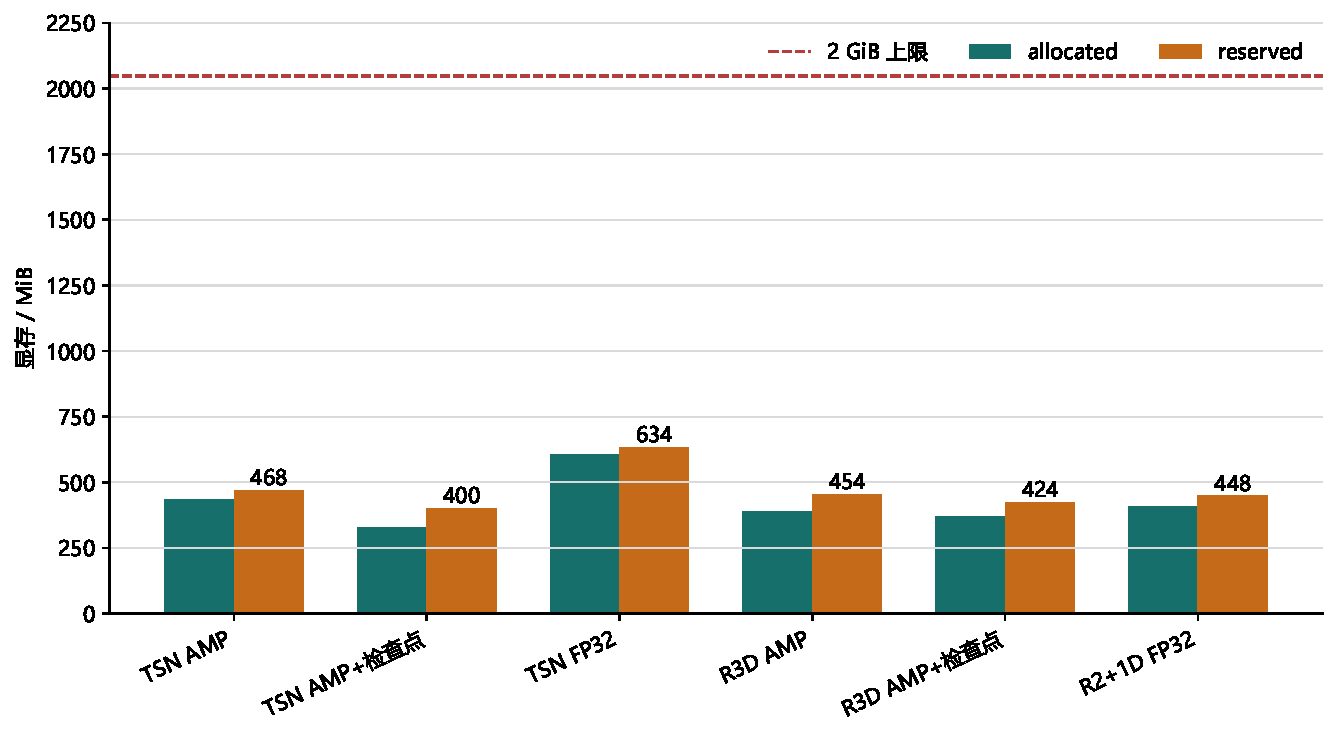
\includegraphics[width=0.93\textwidth]{../../figures/memory_efficiency.pdf}
  \caption{AMP 与梯度检查点的显存峰值对照}
  \label{fig:memory}
\end{figure}

所有单步消融均远低于 2048 MiB。正式实验中最接近上限的是 16 帧时间优先时序头，
其 reserved 峰值为 1912 MiB，仍满足硬门禁。由此可以看出，当输入时间长度增加时，
视频级特征张量和注意力计算会迅速成为主要显存压力。

\subsection{时间与空间投入优先级}

在每视频 65536 个空间像素帧的等成本条件下，16 帧低分辨率的时序头 Top-1 只有
61.71\%，而 4 帧高分辨率的时序头达到 84.19\%。空间优先比时间优先高 22.48
个百分点，同时特征提取 reserved 峰值更低、吞吐更高。图~\ref{fig:budget} 和
表~\ref{tab:budget} 给出了完整对照。

\begin{figure}[H]
  \centering
  \includegraphics[width=0.78\textwidth]{../../figures/time_space_budget.pdf}
  \caption{相同帧像素成本下的时间优先与空间优先结果}
  \label{fig:budget}
\end{figure}

\begin{table}[H]
  \centering
  \caption{时间与空间预算结果}
  \label{tab:budget}
  \begin{tabular}{lccccc}
    \toprule
    配置 & 输入 & Top-1 & Top-5 & 特征峰值/MiB & 吞吐/(video/s) \\
    \midrule
    时间优先 & 16×64×64 & 61.71±0.37\% & 82.76±0.95\% & 298 & 48.68 \\
    空间优先 & 4×128×128 & 84.19±0.10\% & 95.77±0.03\% & 246 & 71.22 \\
    均衡 & 8×112×112 & 82.70±0.54\% & 95.32±0.60\% & 266 & 52.98 \\
    \bottomrule
  \end{tabular}
\end{table}

该结果回答了题目的核心问题。在本实验的预训练、冻结主干和 8 帧主协议附近，
提高空间分辨率比继续增加低分辨率帧更值得投入。时间维并非无效，TSN 时序注意力
相对平均池化仍提高约 1.41 个百分点，但增加帧数必须同时保持足够的空间细节。
